\section{Appendix}


\subsection{Code}
\label{sec:appendix_code}
All the code used in this project is contained within one file. The main function has all the program flow, while the functions introduced above are written in a functional programing manner. 

Code used in this project: 

\lstinputlisting[language=Python]{image_and_spectrum_analyzis.py}

\subsection{Plots not included in the report}
\label{sec:appendix_plots}

%Figure \ref{fig:quantum_efficiency_camera} shows the quantum efficiency of the Bayer mask in the cameras CCD sensor. 
%\begin{figure}[h]
%    \centering
%    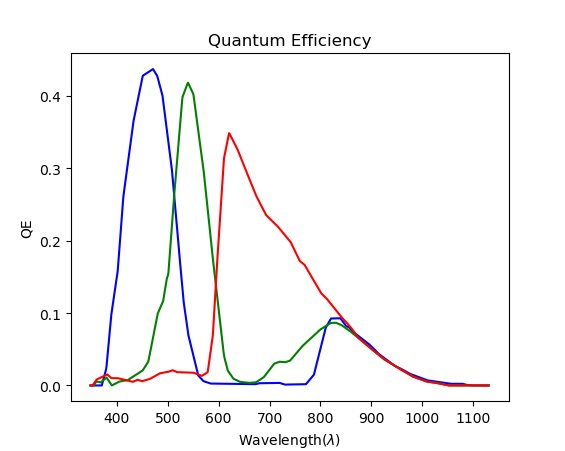
\includegraphics[width=1\textwidth]{Plots/quantum_effiency.png}
%    \caption{The quantum efficiency of the camera}
%    \label{fig:quantum_efficiency_camera}
%\end{figure}


Figure \ref{fig:relative_reflection_around_zero} shows $RR-1$ for nine of the objects being analyzed. 
%TODO3 Figure \ref{fig:relative_reflection_around_zero} shows nine plots, the first one shows the reference spectrum, the spectrum without any objects. The following eight plots shows the Relative Reflectance (\ref{eq:relative_reflectance}), their 
\begin{landscape}
\begin{figure}[t]
    \centering
    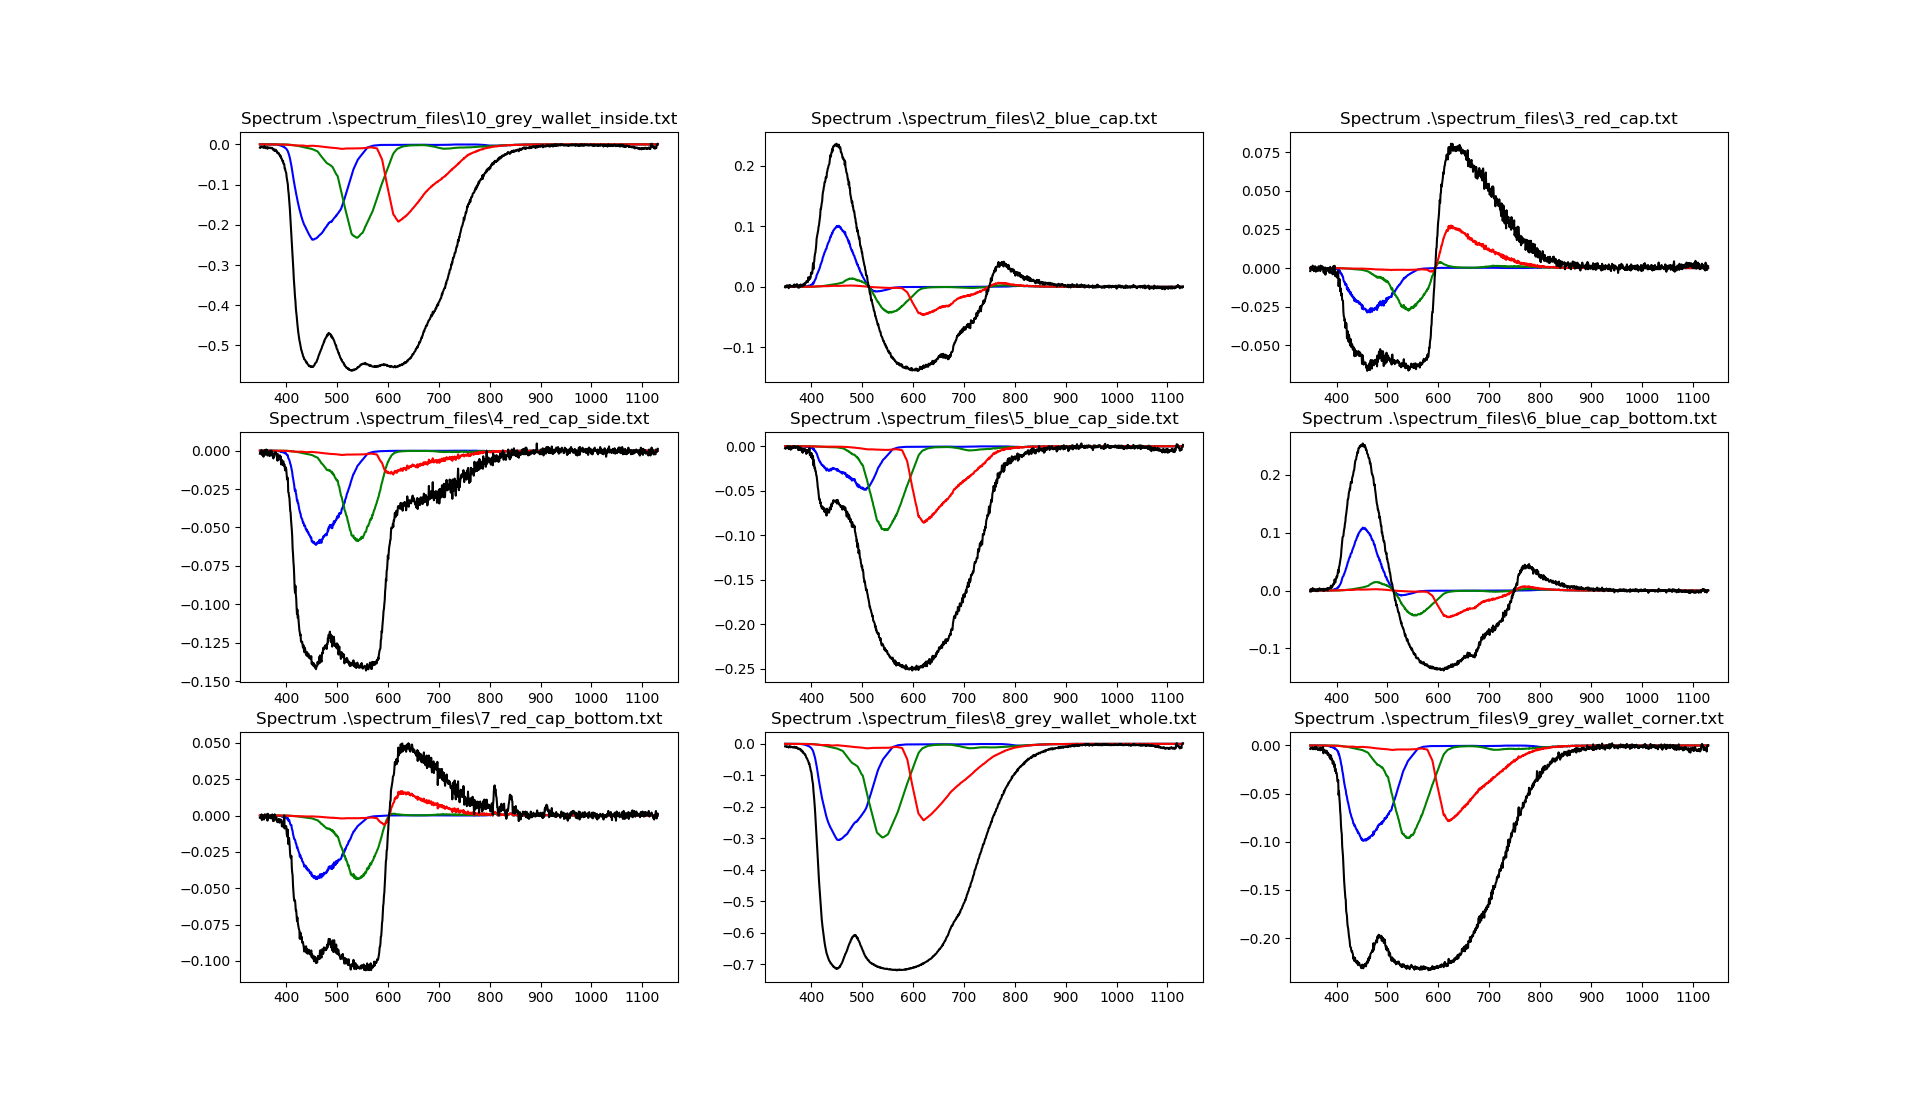
\includegraphics[width=1\paperwidth]{Plots/relative_reflectance_around_zero_with_qe_color_response.png}
    \caption{Relative reflection centered around zero}
    \label{fig:relative_reflection_around_zero}
\end{figure}
\end{landscape}


